\documentclass[10pt, conference]{IEEEtran}

\usepackage{amsmath}
\usepackage{amsfonts}
\usepackage{gensymb}
\usepackage{graphicx}
\usepackage{float}
\usepackage[small,bf]{caption}
\usepackage{subcaption}
\usepackage{url}
\usepackage{color}
\usepackage{epstopdf}
\usepackage{cuted}
\usepackage{tikz}

\usepackage{draftwatermark}

\graphicspath{{figures/},{pdf/},{eps/},{png/}}

\DeclareMathOperator*{\argmin}{argmin}

\renewcommand{\Re}{\operatorname{\textbf{Re}}}
\renewcommand{\Im}{\operatorname{\textbf{Im}}}

\begin{document}

%%%%%%%%%%%%%%%%%%%%%%%%%%%%%%%%%%%%%%%%%%%%%%%%%%
%% TITLE
%%%%%%%%%%%%%%%%%%%%%%%%%%%%%%%%%%%%%%%%%%%%%%%%%%
\title{Optimal Dispatch of Reactive Power for Voltage Regulation and Balancing in Unbalanced Distribution Systems}

%%%%%%%%%%%%%%%%%%%%%%%%%%%%%%%%%%%%%%%%%%%%%%%%%%
%% AUTHORS
%%%%%%%%%%%%%%%%%%%%%%%%%%%%%%%%%%%%%%%%%%%%%%%%%%
\author{
\IEEEauthorblockN{Daniel B. Arnold*, Michael Sankur*, Roel Dobbe**, Kyle Brady**, \\Duncan S. Callaway***, and Alexandra Von Meier**}
\IEEEauthorblockA{*Department of Mechanical Engineering\\
**Department of Electrical Engineering and Computer Science\\
***Energy and Resources Group\\
University of California, Berkeley\\
Berkeley, California 94720\\
(dbarnold, msankur, dobbe, kwbrady, dcal, vonmeier) @berkeley.edu}}

\maketitle

%%%%%%%%%%%%%%%%%%%%%%%%%%%%%%%%%%%%%%%%%%%%%%%%%%
%% SPONSOR FOOTNOTE
%%%%%%%%%%%%%%%%%%%%%%%%%%%%%%%%%%%%%%%%%%%%%%%%%%
\let\thefootnote\relax\footnote{This work was supported in part by the U.S. Department of Energy ARPA-E program (DE-AR0000340).}

%%%%%%%%%%%%%%%%%%%%%%%%%%%%%%%%%%%%%%%%%%%%%%%%%%
%% ABSTRACT
%%%%%%%%%%%%%%%%%%%%%%%%%%%%%%%%%%%%%%%%%%%%%%%%%%
\begin{abstract}
\noindent Optimization of distributed power assets is a powerful tool that has the potential to assist utility efforts to ensure customer voltages are within pre-defined tolerances and to improve distribution system operations. While convex relaxations of Optimal Power Flow (OPF) problems have been proposed for both balanced and unbalanced networks, these approaches do not provide universal convexity guarantees and scale inefficiently as network size and the number of  constraints increase.  In balanced networks, a linearized model of power flow, the LinDistFlow model, has been successfully employed to solve approximate OPF problems quickly and with high degrees of accuracy.  In this work, an extension of the LinDistFlow model is proposed for unbalanced distribution systems, and is  subsequently used to formulate an approximate unbalanced OPF problem that uses VAR assets for voltage  balancing and regulation.  Simulation results on the IEEE 13 node test feeder demonstrate the ability of the unbalanced LinDistFlow model to perform voltage regulation and balance system voltages.
\end{abstract}

%%%%%%%%%%%%%%%%%%%%%%%%%%%%%%%%%%%%%%%%%%%%%%%%%%
%% IEEE KEYWORDS
%%%%%%%%%%%%%%%%%%%%%%%%%%%%%%%%%%%%%%%%%%%%%%%%%%
% \begin{IEEEkeywords}
% Distributed energy resources, Voltage regulation,  Load Following, Model Predictive Control, Distributed Plug Load Control, Battery Storage Optimization
% \end{IEEEkeywords}

\section*{Nomenclature}

% % \noindent $n$ : Number of nodes along feeder \\
% \noindent $\mathcal{P}_{k}$ : Set of phases that exist at node $k$ \\
% \noindent $\mathcal{P}_{jk}$ : Set of phases that exist on line $(j,k)$ \\
% \noindent $V_{k}^{\phi}$ : Voltage phasor at node $k$ on phase $\phi$ \\
% \noindent $\mathbb{V}_{k}$ : Vector of voltage phasors at node $k$ \\
% \noindent $y_{k}^{\phi}$ : Square magnitude of voltage at node $k$ on phase $\phi$ \\ %s.t. $Y_{\phi,k} = \left| V_{\phi,k} \right| ^2$ \\
% \noindent $\mathbb{Y}_{k}$ : Vector of square magnitudes of voltage at node $k$ \\
% \noindent $\delta_{k}^{\phi}$ : Phase angle of voltage phasor at node $k$ on phase $\phi$ \\
% \noindent $Z_{jk}^{\phi \phi}$ : Impedance of segment $(j,k)$ on phase $\phi$ \\
% \noindent $Z_{jk}^{\phi \psi}$ : Impedance of segment $(j,k)$ between phases ($\phi,\psi$) \\
% \noindent $\mathbb{Z}_{jk}$ : Impedance matrix of line segment $(j,k)$ \\
% \noindent $I_{k}^{\phi}$ : Current phasor entering node $k$ on phase $\phi$ \\
% \noindent $\mathbb{I}_{k}$ : Vector of current phasors entering node $k$ \\
% \noindent $i_{k}^{\phi}$ : Load current of phase $\phi$ at node $k$ \\
% \noindent $\mathbf{i}_{k}$ : Vector of load currents at node $k$ \\
% \noindent $S_{k}^{\phi}$ : Phasor of complex power entering node $k$ on phase $\phi$ \\
% \noindent $\mathbb{S}_{k}$ : Vector of complex power phasors entering node $k$ \\
% \noindent $s_{k}^{\phi}$ : Complex load on phase $\phi$ at node $k$ \\
% \noindent $\mathbf{s}_{k}$ : Vector of complex loads at node $k$ \\
% \noindent $u_{k}^{\phi}$ : Inverter real power dispatch on phase $\phi$ at node $k$ \\
% \noindent $v_{k}^{\phi}$ : Inverter VAR dispatch on phase $\phi$ at node $k$
\label{sec:nomenclature}

\section{Introduction}
\label{sec:introduction}

Coordination of a diverse set of Distributed Energy Resources (DER) presents many challenges to utility operators, who strive to ensure power of sufficient quality and quantity is available to retail customers at least cost.  Such assets can vary in size and nature from rooftop PV units and larger PV arrays, to battery storage systems, and demand response resources.  Lack of intelligent management and coordination of DER (distributed PV, specifically) has already resulted in financial impacts for customers and the utility in Hawaii \cite{stewart2013analysis}.  However, DER could, under the correct operational control scenarios, provide numerous benefits to the grid, including voltage support, ancillary services \cite{doe2015ADMS} and, perhaps, new sets of services that were previously infeasible due to lack of controlability or observability.

In distribution systems, it is important to distinguish control strategies based on balanced and unbalanced analysis.  Indeed, a variety of strategies for the management of DER presently exist in which decisions are based on knowledge of balanced distribution system models.  Turitsyn et al. \cite{turitsyn2011options} considered a suite of distributed control strategies for reactive power compensation using four quadrant inverters.  The work of \cite{li2014real} studies distributed voltage regulation in the absence of communication, relying on locally obtained information.  In \cite{robbins2013two}, a two-stage control architecture for voltage regulation is considered where distributed controllers inject power based on local sensitivity measurements.  The authors of \cite{zhang2013local} study local voltage reference tracking with integral-type controllers, based on local voltage measurements.  The authors of \cite{farivar2011inverter} address voltage regulation and loss minimization through solving an Optimal Power Flow (OPF) problem, and address convexity issues using second order cone relaxations.  The work of \cite{lam2012optimal} also considers an OPF approach for voltage regulation in distribution networks by framing the decision-making process as a semidefinite program.  The authors provide conditions under which the semidefinite relaxation of the non-convex power flow problem is tight in balanced circuits. It is worth noting that many of the aforementioned approaches can be traced back to the seminal work of \cite{baran1989optimal}, that introduced nonlinear and linear-approximated recursive branch power flow models.  Finally, several of the authors of this paper have considered solving balanced optimal power flow problems where decisions are made in the absence of a network model \cite{arnold2015model}.

However, as since neither loads nor impedances on all three phases are necessarily close to equal, and individual controllable DER may only be connected to single phases, strategies that consider individual phases as well as their mutual coupling effects need to be considered.  Approaches to coordinate DER in unbalanced distribution systems, while being critical to the practical application in real distribution systems and microgrids \cite{doe2015ADMS}, are much less prevalent in the literature.  
While there is consensus about the physics-based models \cite{kersting2012distribution}, using these in an optimization setting is challenging as the nonlinear nature of power flow equations introduces considerable complexity that can be prohibitive for optimal power flow (OPF) calculations. Perhaps the best known efforts have been put forth by Dall'Anese et. al \cite{dall2012optimization}, \cite{dall2013distributed}, who consider Semi-Definite Program (SDP) relaxations for OPF problems in unbalanced systems, but do not provide conditions under which feasibility and optimality are guaranteed.  In addition to inefficient scaling as the problem size grows, the work of \cite{bitar2014} points out that it becomes more difficult to find a tight relaxation as the ratio of constraints to network buses increases.  A likely reason that more strategies focusing on coordination of distributed energy resources in unbalanced systems do not exist is the lack of suitable linear models that approximate three phase power flow.

A key feature of linear models that makes them so attractive to incorporate into DER control strategies lies in their versatility to enable new types of problems to be formulated and solved.  In our previous works \cite{arnold2015optimal} \cite{sankur2016linear}, we proposed a linearized unbalanced power flow model that can be viewed as an extension of the \emph{LinDistFlow} \cite{baran1989optimal} linear approximation for balanced systems.  This model was incorporated into an OPF designed to balance voltage magnitudes in three phase systems.  Such an activity, to our knowledge, cannot be formulated as an SDP.

Another emerging application to which unbalanced linearized power flow models may be applied (to manage DER) is to enable fast and safe switching of circuit elements in distribution systems.  The ability to island/reconnect microgrids and reconfigure distribution feeders are seen as two important applications of future grids \cite{grid2015}, \cite{quad2015}.  Prior to opening or closing a switch, it is desireable to minimize the voltage phasor difference across the switch to ensure the distribution system is not overly disturbed by large instantenous power flows.  The ability to ``cleanly'' switch elements into and out of a given system could allow for faster restoration of electrical services to critical loads following a disaster, or allow for damaged components to be isolated for repair or replacement.  

While most typical distribution systems do not have the sensing equipment to monitor voltage \emph{phasors}, the growing presence of distribution Phasor Measurement Units (PMUs), indicates that sufficient infrastructure may be in place in future grids to support control activities seeking to regulate feeder voltage phasors.  In fact, a small, but growing, number of control applications that utilize phase angle measurements have started to appear in literature.  The work of \cite{ochoa2010angle} proposed the use of voltage angle measurements to curtail over-generation of renewables.  Additionally, the authors of \cite{wang2013pmu} considered voltage angle thresholds as criteria to connect renewable generation.  Both works refer to this control activity as ``Angle Constrained Active Management'', or ACAM.

In order to enable a control strategy that can regulate voltage phasors, in this work we extend the previously studied model \cite{arnold2015optimal}, \cite{sankur2016linear} which we refer to as the \emph{LinDist3Flow} system, to consider voltage phase angles, thereby allowing OPF formulations to manage voltage phasors rather as opposed to only magnitudes.  

The specific activity studied herein is an OPF formulation that minimizes the voltage phasor difference across an open switch in a distribution system while simultaneously regulating feeder voltage magnitudes to within acceptable limits.  In the event that one of the phasors is uncontrolled (i.e. a reference signal), then this activity can be though of as a voltage phasor tracking problem.  In driving the voltage phasor difference across a circuit element to 0, we ensure that when the switch is closed, only small amounts of power will flow across this element.  In this manner, the switch can be closed without disturbing the rest of the voltage profile in the feeder.  

We first discuss the \emph{Dist3Flow} equations and extend the system to model voltage angles in Section \ref{sec:analysis}.  Here, we also apply simplifying assumptions to the extended \emph{Dist3Flow} system to derive a linear model suitable for incorporation into an optimal power flow formulation (we refer to the linearized system as the \emph{LinDist3Flow} model).  Simulation results of an OPF that uses the \emph{LinDist3Flow} system to track a voltage phasor reference at a specific point in the network, and regulate system voltage magnitudes are presented in Section \ref{sec:simulation_results}.

% of 3-phase complex power flow and introduce linearizations. In \ref{subsec:mag_general}, a model of voltage magnitude on 3-phase unbalanced systems is presented, as are linearizing assumptions, and a special case is discussed in \ref{subsec:mag_nominal}. In \ref{subsec:angle_general}, we derive a nonlinear set of equations relating the phase angle to power injections on a 3-phase network, and discuss linearizing assumptions. A special case of the linearized system is discussed in \ref{subsec:angle_nominal}.
\label{sec:introduction}

\section{Preliminaries}

\setlength{\abovedisplayskip}{-5pt} \setlength{\abovedisplayshortskip}{-5pt}
\setlength{\belowdisplayskip}{0pt} \setlength{\belowdisplayshortskip}{0pt}

Let $T = (H,E)$ denote rooted tree graph representing a balanced radial distribution feeder, where $H$ is the set of nodes of the feeder and the transmission link and $E$ is the set of line segments.  Nodes are indexed by $i = 0,1,\dots,m$, where $m$ is the order (number of nodes) of the distribution feeder, and node 0 denotes the feeder head (or substation).  We treat node 0 as an infinite bus, decoupling interactions in the downstream distribution system from the rest of the grid.  While the substation voltage may evolve over time, we assume this evolution takes place independently of our inverter control action.  For adjacent nodes $j$ and $k$, the current/voltage relationship is captured by KVL and KCL:

\begin{align}
	    \begin{bmatrix}
  		V_{a} \\
  		V_{b} \\
  		V_{c}
  	\end{bmatrix}_{j}
  	&=
  	\begin{bmatrix}
  		V_{a} \\
  		V_{b} \\
  		V_{c}
  	\end{bmatrix}_{k}
  	+
  	\begin{bmatrix}
  		Z_{aa} & Z_{ab} & Z_{ac} \\
  		Z_{ba} & Z_{bb} & Z_{bc} \\
  		Z_{ca} & Z_{cb} & Z_{cc}
  	\end{bmatrix}_{jk}
  	\begin{bmatrix}
  		I_{a} \\
  		I_{b} \\
  		I_{c}
  	\end{bmatrix}_k \label{eq:KVL}
% \end{align}
    \\
% \begin{align}
    \begin{bmatrix}
  		I_{a} \\
  		I_{b} \\
  		I_{c}
  	\end{bmatrix}_{j}
  	&= \begin{bmatrix}
  		i_{a} \\
  		i_{b} \\
  		i_{c}
  	\end{bmatrix}_{j} + \sum_{k:(j,k) \in E}
  	\begin{bmatrix}
  		I_{a} \\
  		I_{b} \\
  		I_{c}
  	\end{bmatrix}_{k}\label{eq:KCL},
\end{align} 

\noindent where $i_{a}$ denotes phase $a$ load current, and $Z_{aa}$ and $Z_{ab}$ are the self impedance for phase $a$ and mutual impedance between phases $a$ and $b$, etc..  We assume that each node serves a complex load in each phase, $s_{\phi,k} = V_{\phi,k}i_{\phi,k}^{*}$ whose real and reactive power components are given by \eqref{eq:pV} and \eqref{eq:qV}, respectively.

\begin{align}
	p_{\phi,k} ( V_{\phi,k} ) & = p_{\phi,k} \left(a_{\phi,k}^{0} + a_{\phi,k}^{1} \left| V_{\phi,k} \right|^2 \right)
    \label{eq:pV}
    \\
    q_{\phi,k} ( V_{\phi,k} ) & = q_{\phi,k} \left(a_{\phi,k}^{0} + a_{\phi,k}^{1} \left| V_{\phi,k} \right|^2 \right) + u_{\phi,k}
    \label{eq:qV}
\end{align}

\noindent where $a_{k}^{0} + a_{k}^{1} = 1$ and are, for simplicity, assumed constant across all phases at each node.  $u_{\phi,k}$ is the reactive power that can be sourced or consumed from a VAR resource on phase $\phi$ at node $k$. In our convention, positive demand denotes power consumption and negative demand is power injected, or supplied, to the grid.  Equations \eqref{eq:KVL}--\eqref{eq:qV} represent the power flow model that will be used to generate simulations in Section \ref{sec:simulation_results}.  

% In this section, we introduce and define several important parameters, approximations, relationships and equations. The constant $\alpha$, extensively used in the study and analysis of power systems, is defined by (\ref{eq:def_alpha}).

% \begin{equation}
% 	\alpha = 1 \angle 120 \degree \quad \alpha^{2} = 1 \angle 240 \degree
%     \label{eq:def_alpha}
% \end{equation}

% In (\ref{eq:VaVbVc}), we introduce an approximation for the quotient of two different phasee voltage phasors at a node. We assume that the magnitude of the phasors for each phase are roughly equivalent at each node. Furthermore, we assume that the phase angle difference is $\pm 120 \degree$ as appropriate. These assumptions are reflected in (\ref{eq:VaVbVc}).

% \begin{equation}
% 	V_{a,k} V_{b,k}^{-1} \approx \alpha \quad V_{b,k} V_{c,k}^{-1} \approx \alpha \quad V_{a,k} V_{c,k}^{-1} \approx \alpha^{2}
%     \label{eq:VaVbVc}
% \end{equation}

% A vector of general values for the three phases at a node is defined by (\ref{eq:def_Xk}). Bold font ($\mathbb{X}$) indicates a vector or matrix, and the subscript $k$ indicates the node. Normal font ($X$) indicates a value at a particular phase. The first subscript indicates the phase, with $\phi$ being a general phase, and $a,b,c$ the actual phase. The second subscript $k$, if present, indicates the node of the individual value or vector.

% \begin{equation}
% 	\mathbb{X}_{k}
%     =
%     \begin{bmatrix}
%     X_{a,k} \\
%     X_{b,k} \\
%     X_{c,k} \\
%     \end{bmatrix}
%     =
%     \begin{bmatrix}
%     X_{a} \\
%     X_{b} \\
%     X_{c} \\
%     \end{bmatrix}_{k}
%     \label{eq:def_Xk}
% \end{equation}

% The power entering a node on a phase is defined as the phase voltage at the node multiplied by the complex conjugate of the phase current entering the node, as in (\ref{eq:def_Sk}). 

% \begin{equation}
% 	S_{\phi,k} = V_{\phi,k} I_{\phi,k}^{*}
%     \label{eq:def_Sk}
% \end{equation}

% The squared magnitude of a voltage phasor is given by (\ref{eq:def_Yk}).

% \begin{equation}
% 	y_{\phi,k} = \left| V_{\phi,k} \right|^2 = V_{\phi,k} V_{\phi,k}^*
%     \label{eq:def_Yk}
% \end{equation}

% Kirchoff's Voltage Law for a three phase line between two nodes is given by (\ref{eq:kvl_3phase}), and is represented in its compact and expanded form. In all equations we assume node $k-1$ is immediately upstream (toward the feeder head) of node $k$.

% \begin{equation}
% \begin{gathered}
% 	\mathbb{V}_{k-1} = \mathbb{V}_{k} + \mathbb{Z}_{k} \mathbb{I}_{k} \\
%     \begin{bmatrix}
%   		V_{a} \\
%   		V_{b} \\
%   		V_{c}
%   	\end{bmatrix}_{k-1}
%   	=
%   	\begin{bmatrix}
%   		V_{a} \\
%   		V_{b} \\
%   		V_{c}
%   	\end{bmatrix}_{k}
%   	+
%   	\begin{bmatrix}
%   		Z_{aa} & Z_{ab} & Z_{ac} \\
%   		Z_{ba} & Z_{bb} & Z_{bc} \\
%   		Z_{ca} & Z_{cb} & Z_{cc}
%   	\end{bmatrix}_k
%   	\begin{bmatrix}
%   		I_{a} \\
%   		I_{b} \\
%   		I_{c}
%   	\end{bmatrix}_k
% \end{gathered}
% \label{eq:kvl_3phase}
% \end{equation}

% % \begin{figure}[t]
% % 	\centering
% % 	\includegraphics[width=0.5\textwidth, clip, trim = 2.875in 2.875in 2.375in 2.125in]{kvl.pdf}
% %     \caption{Nodes $k-1$ and $k$ with line impedances and power entering the phases at node $k$ shown.}
% % 	\label{fig:kvl_3phase}
% % \end{figure}


\label{sec:preliminaries}

\subsection{Linearized Model for Unbalanced 3-phase Power Flow}

\setlength{\abovedisplayskip}{-5pt}
\setlength{\belowdisplayskip}{-0pt}

In this section, we derive a linear approximation of three phase power flow.  This model can be thought of as an extension of the \emph{LinDistFlow} model to unbalanced circuits.  Consider two adjacent nodes of the distribution feeder, $(j,k) \in H$.  We begin by expressing \eqref{eq:KVL}--\eqref{eq:KCL} in vector form:

\begin{align}
	\mathbb{V}_{j} &= \mathbb{V}_{k} + \mathbb{Z}_{k} \mathbb{I}_{k} \label{eq:KVL_compact} \\
    \mathbb{I}_{j} &=  \mathbf{i}_{j}+ \sum_{k:(j,k)\in E}\mathbb{I}_{k} \label{eq:KCL_compact}.
\end{align}

% \noindent where

% \begin{align}
% 	\mathbb{V}_{j} &= \begin{bmatrix}
%     					V_{a} \\
%     					V_{b} \\
%     					V_{c} \\
%     					\end{bmatrix}_{j}
%     \mathbb{I}_{j} = \begin{bmatrix}
%     					I_{a} \\
%     					I_{b} \\
%     					I_{c} \\
%     					\end{bmatrix}_{j}
%     \mathbf{i}_{j} = \begin{bmatrix}
%     					i_{a} \\
%     					i_{b} \\
%     					i_{c} \\
%     					\end{bmatrix}_{j} \nonumber \\
%     \mathbb{Z}_{jk} &=\begin{bmatrix}
%   		Z_{aa} & Z_{ab} & Z_{ac} \\
%   		Z_{ba} & Z_{bb} & Z_{bc} \\
%   		Z_{ca} & Z_{cb} & Z_{cc}
%   	\end{bmatrix}_{jk} \nonumber
% \end{align}

We now right multiply each side of \eqref{eq:KVL_compact} by its complex conjugate and right multiply both sides of ~\eqref{eq:KCL_compact} by $\mathbb{V}_{j}^{*}$ and take the complex conjugate, resulting in:

\begin{align}
	\mathbb{V}_{j} \mathbb{V}_{j}^*  & =  \mathbb{V}_{k} \mathbb{V}_{k}^* + \mathbb{Z}_{k} \mathbb{I}_{k} \mathbb{V}_{k}^* + \mathbb{V}_{k} \mathbb{I}_{k}^{*} \mathbb{Z}_{k}^{*} + \mathbb{Z}_{k} \mathbb{I}_{k} \mathbb{I}_{k}^{*} \mathbb{Z}_{k}^{*} \nonumber \\
    & = \mathbb{V}_{k} \mathbb{V}_{k}^* + 2 \Re \left\{\mathbb{V}_{k} \mathbb{I}_{k}^{*} \mathbb{Z}_{k}^{*} \right\} + \mathbb{Z}_{k} \mathbb{I}_{k} \mathbb{I}_{k}^{*} \mathbb{Z}_{k}^{*}
\label{eq:mag_1},
\end{align}

% \noindent and

\begin{align}
	\mathbb{V}_{j}\mathbb{I}_{j}^{*} &= \mathbb{V}_{j}\mathbf{i}_{j}^{*} + \sum_{k:(j,k) \in E} \left(\mathbb{V}_{k} + \mathbb{Z}_{k}\mathbb{I}_{k}\right)\mathbb{I}_{k}^{*} \label{eq:pow_1}.
\end{align}

Similar to the derivation of the \emph{LinDistFlow} system, we neglect loss terms in \eqref{eq:mag_1}--\eqref{eq:pow_1}, which yields:

\begin{align}
    \mathbb{V}_{j}\mathbb{V}_{j}^{*} &\approx \mathbb{V}_{k} \mathbb{V}_{k}^* + 2 \Re \left\{\mathbb{V}_{k} \mathbb{I}_{k}^{*} \mathbb{Z}_{k}^{*} \right\} \label{eq:mag_2} \\
	\mathbb{V}_{j}\mathbb{I}_{j}^{*} &\approx \mathbb{V}_{j}\mathbf{i}_{j}^{*} + \sum_{k:(j,k) \in E} \mathbb{V}_{k}\mathbb{I}_{k}^{*} \label{eq:pow_2}.
\end{align}

\noindent where \eqref{eq:mag_1}--\eqref{eq:pow_1} are $3\times 3$ matrix equations. Focusing our attention first on \eqref{eq:pow_1}, we apply the power equation $S_{\phi,k} = V_{\phi,k}I_{\phi,k}^{*}$ to the diagonal elements and collect these into the vector equation:

\begin{align}
	\mathbb{S}_{j} \approx \mathbf{s}_{j} + \sum_{k:(j,k) \in E} \mathbb{S}_{k} \label{eq:pow_3}
\end{align}

Returning attention to \eqref{eq:mag_2}, we expand $\mathbb{I}_{k}$ according to $S_{\phi,k} = V_{\phi,k}I_{\phi,k}^{*}$, resulting in:

\begin{equation}
	\begin{aligned}
		\mathbb{V}_{j} & \mathbb{V}_{j}^{*} \approx \mathbb{V}_{k} \mathbb{V}_{k}^{*} + \\
    	& 2 \Re \left\{ \mathbb{V}_{k}
    	\begin{bmatrix}
    		S_{a} V_{a}^{-1} & S_{b} V_{b}^{-1} & S_{c} V_{c}^{-1}
    	\end{bmatrix}_k
    	\mathbb{Z}_{jk}^* \right\}
    \end{aligned}
    \label{eq:mag_3}
\end{equation}

\noindent which is equivalent to:

\begin{equation}
	\begin{aligned}
		\mathbb{V}_{j} & \mathbb{V}_{j}^{*} \approx \mathbb{V}_{k} \mathbb{V}_{k}^{*} + \\
    	& 2 \Re \left\{
    	\begin{bmatrix}
    		S_{a} & V_{a} S_{b} V_{b}^{-1} & V_{a} S_{c} V_{c}^{-1} \\
    		V_{b} S_{a} V_{a}^{-1} & S_{b} & V_{b} S_{c} V_{c}^{-1} \\
    		V_{c} S_{a} V_{a}^{-1} & V_{c} S_{b} V_{b}^{-1} & S_{c}
    	\end{bmatrix}_k
    	\mathbb{Z}_{jk}^* \right\}
    \end{aligned}
    \label{eq:mag_4}
\end{equation}

\setlength{\abovedisplayskip}{-5pt}
\setlength{\belowdisplayskip}{-0pt}

Note that even after neglecting the loss terms, \eqref{eq:mag_4} is still nonlinear.  To further simplify the system, we adopt an approximation that assumes the ratio of voltage phasors are constant:

% \setlength{\abovedisplayskip}{-6pt} \setlength{\abovedisplayshortskip}{-6pt}
% \setlength{\belowdisplayskip}{-0pt} \setlength{\belowdisplayshortskip}{-0pt}

\begin{equation}
	V_{a,k} V_{b,k}^{-1} \approx \alpha \quad V_{b,k} V_{c,k}^{-1} \approx \alpha \quad V_{a,k} V_{c,k}^{-1} \approx \alpha^{2}
    \label{eq:VaVbVc}
\end{equation}

\noindent where

\begin{align}
	\alpha = &1 \angle 120 \degree = \frac{-1 + j\sqrt{3}}{2}, \quad \alpha^{2} = 1 \angle 240 \degree = -\frac{1 + j\sqrt{3}}{2}.
    \label{eq:alpha}
\end{align}

The simplification of the quotient of the voltage phasors according to \eqref{eq:VaVbVc}--\eqref{eq:alpha} transforms \eqref{eq:mag_4} into:
	
\begin{equation}
	\mathbb{V}_{j} \mathbb{V}_{j}^{*} \approx \mathbb{V}_{k} \mathbb{V}_{k}^{*} + 2 \Re \left\{
    \begin{bmatrix}
    	S_{a} & \alpha S_{b} & \alpha^{2} S_{c} \\
    	\alpha^{2} S_{a} & S_{b} & \alpha S_{c} \\
    	\alpha S_{a} & \alpha^{2} S_{b} & S_{c}
    \end{bmatrix}_k
    \mathbb{Z}_{jk}^* \right\}
    \label{eq:mag_5}
\end{equation}

Although ~\eqref{eq:mag_5} is a $3\times 3$ matrix equation, we are intertested only in the diagonal elements, which we gather and place into $3 \times 1$ vectors resulting in \eqref{eq:mag_6}:

\begin{align}
	\mathbb{Y}_{j} &\approx \mathbb{Y}_{k} +\nonumber \\
    & 2 \Re \left\{
    \begin{bmatrix}
    	Z_{aa,jk}^{*} S_{a,k}  + \alpha Z_{ab,jk}^{*} S_{b,k}  + \alpha^{2} Z_{ac,jk}^{*} S_{c,k} \\
    	\alpha^{2} Z_{ba,jk}^{*} S_{a,k} + Z_{bb,jk}^{*} S_{b,k} + \alpha Z_{bc,jk}^{*} S_{c,k} \\
    	\alpha Z_{ca,jk}^{*} S_{a,k} + \alpha^{2} Z_{cb,jk}^{*} S_{b,k} + Z_{cc,jk}^{*} S_{c,k}
    \end{bmatrix}
	\right\}
    \label{eq:mag_6},
\end{align}

\noindent  where we have defined the vector of the square of voltage magnitudes in phases $a,b,c$ as $\mathbb{Y}_{k} = \begin{bmatrix} y_{a} & y_{b} & y_{c} \end{bmatrix}_{k}^{T}$.  The $3 \times 1$ vector inside the $\Re$ operator can be broken up into a $3 \times 3$ matrix of impedances for line segment $(j,k)$ and a $3 \times 1$ vector of node $k$ power injections, as is shown in \eqref{eq:mag_7}.

\begin{align}
	\mathbb{Y}_{j} &\approx \mathbb{Y}_{k} + \nonumber \\
    &2 \Re \left\{
    \begin{bmatrix}
    	Z_{aa}^{*} & \alpha Z_{ab}^{*} & \alpha^{2} Z_{ac}^{*} \\
    	\alpha^{2} Z_{ba}^{*} & Z_{bb}^{*} & \alpha Z_{bc}^{*} \\
    	\alpha Z_{ca}^{*} & \alpha^{2} Z_{cb}^{*} & Z_{cc}^{*}
    \end{bmatrix}_{jk}
    \begin{bmatrix}
    	S_{a} \\ S_{b} \\ S_{c}
    \end{bmatrix}_{k}
	\right\}
    \label{eq:mag_7}
\end{align}

Viewed in this form, the approximation to the ratio of voltage phasors essentially introduces $\pm 120 \degree$ rotations of the cross-phase impedances. Expanding the impedance matrix entries as $Z_{\phi \psi,k} = r_{\phi, \psi,k} + j x_{\phi, \psi,k}$, the complex power as $S_{\phi,k} = P_{\phi,k} + j Q_{\phi,k}$, and using the definition of $\alpha$, it can be shown that \eqref{eq:mag_7} simplifies into the following linear matrix equation:

\begin{align}
	\mathbb{Y}_{j} &\approx \mathbb{Y}_{k} - \mathbb{M}_{jk}^{P} \mathbb{P}_{k} - \mathbb{M}_{jk}^{Q} \mathbb{Q}_{k} \label{eq:mag_8}
\end{align}

\noindent where

% \begin{align}
% 	\mathbb{M}_{jk}^{P} &=
% 	\begin{bmatrix}
% 		2 r_{aa} & -r_{ab} + \sqrt{3} x_{ab} & -r_{ac} - \sqrt{3} x_{ac} \\
% 		-r_{ba} - \sqrt{3} x_{ba} & 2 r_{bb} & -r_{bc} + \sqrt{3} x_{bc} \\
% 		-r_{ca} + \sqrt{3} x_{ca} & -r_{cb} - \sqrt{3} x_{cb} & 2 r_{cc}
% 	\end{bmatrix}_{jk} \\
% 	\mathbb{M}_{jk}^{Q} &=
% 	\begin{bmatrix}
% 		2 x_{aa} & -\sqrt{3} r_{ab} - x_{ab} & \sqrt{3} r_{ac} - x_{ac} \\
% 		\sqrt{3} r_{ba} - x_{ba} & 2 x_{bb} & -\sqrt{3} r_{bc} - x_{bc} \\
% 		-\sqrt{3} r_{ca} - x_{ca} & \sqrt{3} r_{cb} - x_{cb} & 2 x_{cc}
% 	\end{bmatrix}_{jk}
% \end{align}

\begin{align}
	\mathbb{M}_{jk}^{P} &=
	\begin{bmatrix}
		-2 r_{aa} & r_{ab} - \sqrt{3} x_{ab} & r_{ac} + \sqrt{3} x_{ac} \\
		r_{ba} + \sqrt{3} x_{ba} & -2 r_{bb} & r_{bc} - \sqrt{3} x_{bc} \\
		r_{ca} - \sqrt{3} x_{ca} & r_{cb} + \sqrt{3} x_{cb} & -2 r_{cc}
	\end{bmatrix}_{jk} \label{eq:M}\\
	\mathbb{M}_{jk}^{Q} &=
	\begin{bmatrix}
		-2 x_{aa} & x_{ab} + \sqrt{3} r_{ab} & x_{ac} - \sqrt{3} r_{ac} \\
		x_{ba} -\sqrt{3} r_{ba} & -2 x_{bb} & x_{bc} + \sqrt{3} r_{bc}\\
		x_{ca} + \sqrt{3} r_{ca} & x_{cb} -\sqrt{3} r_{cb} & -2 x_{cc}
	\end{bmatrix}_{jk} \label{eq:N}.
\end{align}

We now restate ~\eqref{eq:pow_3} for completeness:

\begin{align}
	\mathbb{S}_{j} \approx \mathbf{s}_{j} + \sum_{k:(j,k) \in E} \mathbb{S}_{k} \label{eq:pow_4}
\end{align}

Equations ~\eqref{eq:mag_8}--\eqref{eq:pow_4} represent a linearized model of unbalanced distribution power flow that maps node $k$ real and reactive power injections into squared voltage magnitude differences. As the system shows, power contribution in all three phases collectively influence each phase's squared voltage magnitude difference.  It is easily verified that a reduction to a single phase network results in the \emph{LinDistFlow} model discussed in \cite{baran1989optimal}.

% It is clear that using \eqref{eq:KVL} to propagate voltage throughout the feeder would lead to a system of nonlinear equations to find the voltage magnitudes. This approximation bypasses these nonlinearities and does not affect convexity.


%%%%%%%%%%%%%%%%%%%%%%%%%%%%%%%%%%%%%%%%%%%%%%%%%%%%%%%%%%%%%%%%%%%%%%%%%%%%%%%%%%%

% In this section, we introduce and define several important parameters, approximations, relationships and equations. The constant $\alpha$, extensively used in the study and analysis of power systems, is defined by (\eqref{eq:def_alpha}).

% \begin{equation}
% 	\alpha = 1 \angle 120 \degree \quad \alpha^{2} = 1 \angle 240 \degree
%     \label{eq:def_alpha}
% \end{equation}

% In (\eqref{eq:VaVbVc}), we introduce an approximation for the quotient of two different phasee voltage phasors at a node. We assume that the magnitude of the phasors for each phase are roughly equivalent at each node. Furthermore, we assume that the phase angle difference is $\pm 120 \degree$ as appropriate. These assumptions are reflected in (\eqref{eq:VaVbVc}).

% \begin{equation}
% 	V_{a,k} V_{b,k}^{-1} \approx \alpha \quad V_{b,k} V_{c,k}^{-1} \approx \alpha \quad V_{a,k} V_{c,k}^{-1} \approx \alpha^{2}
%     \label{eq:VaVbVc}
% \end{equation}

% A vector of general values for the three phases at a node is defined by (\eqref{eq:def_Xk}). Bold font ($\mathbb{X}$) indicates a vector or matrix, and the subscript $k$ indicates the node. Normal font ($X$) indicates a value at a particular phase. The first subscript indicates the phase, with $\phi$ being a general phase, and $a,b,c$ the actual phase. The second subscript $k$, if present, indicates the node of the individual value or vector.

% \begin{equation}
% 	\mathbb{X}_{k}
%     =
%     \begin{bmatrix}
%     X_{a,k} \\
%     X_{b,k} \\
%     X_{c,k} \\
%     \end{bmatrix}
%     =
%     \begin{bmatrix}
%     X_{a} \\
%     X_{b} \\
%     X_{c} \\
%     \end{bmatrix}_{k}
%     \label{eq:def_Xk}
% \end{equation}

% The power entering a node on a phase is defined as the phase voltage at the node multiplied by the complex conjugate of the phase current entering the node, as in (\eqref{eq:def_Sk}). 

% \begin{equation}
% 	S_{\phi,k} = V_{\phi,k} I_{\phi,k}^{*}
%     \label{eq:def_Sk}
% \end{equation}

% The squared magnitude of a voltage phasor is given by (\eqref{eq:def_Yk}).

% \begin{equation}
% 	y_{\phi,k} = \left| V_{\phi,k} \right|^2 = V_{\phi,k} V_{\phi,k}^*
%     \label{eq:def_Yk}
% \end{equation}

% Kirchoff's Voltage Law for a three phase line between two nodes is given by (\eqref{eq:kvl_3phase}), and is represented in its compact and expanded form. In all equations we assume node $k-1$ is immediately upstream (toward the feeder head) of node $k$.

% % \begin{equation}
% % \begin{gathered}
% % 	\mathbb{V}_{k-1} = \mathbb{V}_{k} + \mathbb{Z}_{k} \mathbb{I}_{k} \\
% %     \begin{bmatrix}
% %   		V_{a} \\
% %   		V_{b} \\
% %   		V_{c}
% %   	\end{bmatrix}_{k-1}
% %   	=
% %   	\begin{bmatrix}
% %   		V_{a} \\
% %   		V_{b} \\
% %   		V_{c}
% %   	\end{bmatrix}_{k}
% %   	+
% %   	\begin{bmatrix}
% %   		Z_{aa} & Z_{ab} & Z_{ac} \\
% %   		Z_{ba} & Z_{bb} & Z_{bc} \\
% %   		Z_{ca} & Z_{cb} & Z_{cc}
% %   	\end{bmatrix}_k
% %   	\begin{bmatrix}
% %   		I_{a} \\
% %   		I_{b} \\
% %   		I_{c}
% %   	\end{bmatrix}_k
% % \end{gathered}
% % \label{eq:kvl_3phase}
% % \end{equation}

% % \begin{figure}[t]
% % 	\centering
% % 	\includegraphics[width=0.5\textwidth, clip, trim = 2.875in 2.875in 2.375in 2.125in]{kvl.pdf}
% %     \caption{Nodes $k-1$ and $k$ with line impedances and power entering the phases at node $k$ shown.}
% % 	\label{fig:kvl_3phase}
% % \end{figure}


% % \begin{equation}
% % 	y_{\phi,k-1} = f \left( \mathbb{Y}_{k} , \mathbb{P}_{k}, \mathbb{Q}_{k} \right)
% % \end{equation}

% We start by considering (\eqref{eq:kvl_3phase}), and right multiply each side by their complex conjugate as in (\eqref{eq:mag_1}). Though this results in $3 \times 3$ matrices in (\eqref{eq:mag_1}), we are only interested in the entries on the diagonals of each matrix, which represent each row of the (\eqref{eq:kvl_3phase}) multiplied by its complex conjugate. Adding complex conjugates results in the second row of (\eqref{eq:mag_1}).

% % \setlength{\abovedisplayskip}{-5pt} \setlength{\abovedisplayshortskip}{-5pt}
% % \setlength{\belowdisplayskip}{-5pt} \setlength{\belowdisplayshortskip}{-5pt}

% \begin{equation}
% \begin{aligned}
% 	\mathbb{V}_{j} \mathbb{V}_{j}^*  & =  \mathbb{V}_{k} \mathbb{V}_{k}^* + \mathbb{Z}_{k} \mathbb{I}_{k} \mathbb{V}_{k}^* + \mathbb{V}_{k} \mathbb{I}_{k}^{*} \mathbb{Z}_{k}^{*} + \mathbb{Z}_{k} \mathbb{I}_{k} \mathbb{I}_{k}^{*} \mathbb{Z}_{k}^{*} \\
%     & = \mathbb{V}_{k} \mathbb{V}_{k}^* + 2 \Re \left\{\mathbb{V}_{k} \mathbb{I}_{k}^{*} \mathbb{Z}_{k}^{*} \right\} + \mathbb{Z}_{k} \mathbb{I}_{k} \mathbb{I}_{k}^{*} \mathbb{Z}_{k}^{*}
% \end{aligned}
% \label{eq:mag_1}
% \end{equation}

% Voltage constraints dictate that feeder node voltage be within a $\pm 5 \%$ range of 1 pu, such that $0.95 \le \left| V_{\phi,k} \right| \le 1.05 \quad \forall \phi, k$. The magnitudes of line and mutual impedances are generally much smaller than 1, the magnitudes of current phasors are generally smaller than $1$. Normal values of impedance and current magnitude are such that $\left| Z_{\phi\phi} \right| \le 0.1$, $\left| Z_{\phi\psi} \right| \le 0.1$, and $\left| I_{\phi} \right| \le 0.5$. Thus approximate magnitudes of elements of $\mathbb{V}_{k} \mathbb{I}_{k}^{*} \mathbb{Z}_{k}^{*}$ and $\mathbb{Z}_{k} \mathbb{I}_{k} \mathbb{I}_{k}^{*} \mathbb{Z}_{k}^{*}$ are shown the first and second row of (\eqref{eq:mag_approx}), respectively.

% \begin{equation}
% \begin{aligned}
% 	& \left| V_{a,k} Z_{aa,k}^* I_{a,k}^* \right| = \left| V_{a,k} \right| \left| Z_{aa,k} \right| \left| I_{a,k} \right| \approx 0.01 \\
%     & \left| Z_{aa,k} I_{a,k} Z_{ab,k}^* I_{b,k}^* \right| = \left| Z_{aa,k} \right| \left| I_{a,k} \right| \left| Z_{ab,k} \right| \left| I_{b,k} \right| \approx 0.0001
% \end{aligned}
% \label{eq:mag_approx}
% \end{equation}

% By (\eqref{eq:mag_approx}), higher order terms such as $\left| Z_{aa,k} I_{a,k} \right|^2$ and $Z_{aa,k} I_{a,k} Z_{ab,k}^* I_{b,k}^*$ which are components of $\mathbb{Z}_{k} \mathbb{I}_{k} \mathbb{I}_{k}^* \mathbb{Z}_{k}^*$ are of negligible magnitude compared to other terms such as $V_{a,k} Z_{aa,k}^* I_{a,k}^*$, which is a component of $\mathbb{V}_{k} \mathbb{I}_{k}^* \mathbb{Z}_{k}^*$. Treating higher order terms of $\mathbb{Z}_{k} \mathbb{I}_{k} \mathbb{I}_{k}^{*} \mathbb{Z}_{k}^{*}$ as negligible simplifies (\eqref{eq:mag_1}) to (\eqref{eq:mag_2}).

% \begin{equation}
% 	\mathbb{V}_{j} \mathbb{V}_{j}^{*} = \mathbb{V}_{k} \mathbb{V}_{k}^{*} + 2 \Re \left\{ \mathbb{V}_{k} \mathbb{I}_{k}^{*} \mathbb{Z}_{k}^{*} \right\}
%     \label{eq:mag_2}
% \end{equation}

% We take advantage (\eqref{eq:def_Sk}) to replace the current phasors in (\eqref{eq:mag_2}), as in (\eqref{eq:mag_3}).

% \begin{equation}
% 	\begin{aligned}
% 		\mathbb{V}_{j} & \mathbb{V}_{j}^{*} = \mathbb{V}_{k} \mathbb{V}_{k}^{*} + \ldots \\
%     	& 2 \Re \left\{ \mathbb{V}_{k}
%     	\begin{bmatrix}
%     		S_{a} V_{a}^{-1} & S_{b} V_{b}^{-1} & S_{c} V_{c}^{-1}
%     	\end{bmatrix}_k
%     	\mathbb{Z}_{jk}^* \right\}
%     \end{aligned}
%     \label{eq:mag_3}
% \end{equation}

% \begin{equation}
% 		\mathbb{V}_{j} \mathbb{V}_{j}^{*} = \mathbb{V}_{k} \mathbb{V}_{k}^{*} +
%     	2 \Re \left\{ \mathbb{V}_{k}
%     	\begin{bmatrix}
%     		S_{a} V_{a}^{-1} & S_{b} V_{b}^{-1} & S_{c} V_{c}^{-1}
%     	\end{bmatrix}_k
%     	\mathbb{Z}_{jk}^* \right\}
%     \label{eq:mag_3}
% \end{equation}

% Multiplying the first two matrices results in (\eqref{eq:mag_4}), and using (\eqref{eq:VaVbVc}) gives (\eqref{eq:mag_5}).

% % \begin{equation}
% % 	\mathbb{Y}_{k-1} = \mathbb{Y}_{k} + 2 \Re \left\{
% %     \begin{bmatrix}
% %     	S_{a,k} & V_{a,k} S_{b,k} V_{b,k}^{-1} & V_{a,k} S_{c,k} V_{c,k}^{-1} \\
% %     	V_{b,k} S_{a,k} V_{a,k}^{-1} & S_{b,k} & V_{b,k} S_{c,k} V_{c,k}^{-1} \\
% %     	V_{c,k} S_{a,k} V_{a,k}^{-1} & V_{c,k} S_{b,k} V_{b,k}^{-1} & S_{c,k}
% %     \end{bmatrix}
% %     \mathbb{Z}_{k}^* \right\} \\
% %     \label{eq:mag_4}
% % \end{equation}

% \begin{equation}
% 	\begin{aligned}
% 		\mathbb{V}_{j} & \mathbb{V}_{j}^{*} = \mathbb{V}_{k} \mathbb{V}_{k}^{*} + \ldots \\
%     	& 2 \Re \left\{
%     	\begin{bmatrix}
%     		S_{a} & V_{a} S_{b} V_{b}^{-1} & V_{a} S_{c} V_{c}^{-1} \\
%     		V_{b} S_{a} V_{a}^{-1} & S_{b} & V_{b} S_{c} V_{c}^{-1} \\
%     		V_{c} S_{a} V_{a}^{-1} & V_{c} S_{b} V_{b}^{-1} & S_{c}
%     	\end{bmatrix}_k
%     	\mathbb{Z}_{jk}^* \right\}
%     \end{aligned}
%     \label{eq:mag_4}
% \end{equation}
	
% \begin{equation}
% 	\mathbb{V}_{j} \mathbb{V}_{j}^{*} = \mathbb{V}_{k} \mathbb{V}_{k}^{*} + 2 \Re \left\{
%     \begin{bmatrix}
%     	S_{a} & \alpha S_{b} & \alpha^{2} S_{c} \\
%     	\alpha^{2} S_{a} & S_{b} & \alpha S_{c} \\
%     	\alpha S_{a} & \alpha^{2} S_{b} & S_{c}
%     \end{bmatrix}_k
%     \mathbb{Z}_{jk}^* \right\}
%     \label{eq:mag_5}
% \end{equation}

% By multiplying the vectors by their complex conjugate to obtain matrices, multiplying the two matrices inside the $\Re$ operator together, and collecting the diagonal elements of all matrices and placing them into vectors gives (\eqref{eq:mag_6}). Here we use define the vector of phase square voltage magnitude as $\mathbb{Y}_{k} = \begin{bmatrix} y_{a,k} & y_{b,k} & y_{c,k} \end{bmatrix}^{T}$.

% \begin{equation}
% 	\mathbb{Y}_{j} = \mathbb{Y}_{k} + 2 \Re \left\{
%     \begin{bmatrix}
%     	Z_{aa}^{*} S_{a}  + \alpha Z_{ab}^{*} S_{b}  + \alpha^{2} Z_{ac}^{*} S_{c} \\
%     	\alpha^{2} Z_{ba}^{*} S_{a} + Z_{bb}^{*} S_{b} + \alpha Z_{bc}^{*} S_{c} \\
%     	\alpha Z_{ca}^{*} S_{a} + \alpha^{2} Z_{cb}^{*} S_{b} + Z_{cc}^{*} S_{c}
%     \end{bmatrix}_k
% 	\right\}
%     \label{eq:mag_6}
% \end{equation}

% The matrix inside the $\Re$ operator can be broken into a $3 \times 3$ matrix and a vector of node complex power, as in (\eqref{eq:mag_7}).

% \begin{equation}
% 	\mathbb{Y}_{j}= \mathbb{Y}_{k} + 2 \Re \left\{
%     \begin{bmatrix}
%     	Z_{aa}^{*} & \alpha Z_{ab}^{*} & \alpha^{2} Z_{ac}^{*} \\
%     	\alpha^{2} Z_{ba}^{*} & Z_{bb}^{*} & \alpha Z_{bc}^{*} \\
%     	\alpha Z_{ca}^{*} & \alpha^{2} Z_{cb}^{*} & Z_{cc}^{*}
%     \end{bmatrix}_{jk}
%     \begin{bmatrix}
%     	S_{a} \\ S_{b} \\ S_{c}
%     \end{bmatrix}_{jk}
% 	\right\}
%     \label{eq:mag_7}
% \end{equation}

% Expanding the impedance matrix entries as $Z_{\phi \psi,k} = r_{\phi, \psi,k} + j x_{\phi, \psi,k}$, the complex power as $S_{\phi,k} = P_{\phi,k} + j Q_{\phi,k}$, the constant $\alpha$ as  $\alpha = \frac{1}{2}(1 + j \sqrt{3})$, and $\alpha^2 = \frac{1}{2}(1 - j \sqrt{3})$, it can be shown that (\eqref{eq:mag_7}) simplifies to (\eqref{eq:mag_8}).

% \begin{equation}
% \begin{gathered}
% 	\mathbb{Y}_{j} = \mathbb{Y}_{k} + \mathbb{M}_{jk}^{P} \mathbb{P}_{k} + \mathbb{M}_{jk}^{Q} \mathbb{Q}_{k} \\
% 	\mathbb{M}_{jk}^{P} =
% 	\begin{bmatrix}
% 		2 r_{aa} & -r_{ab} + \sqrt{3} x_{ab} & -r_{ac} - \sqrt{3} x_{ac} \\
% 		-r_{ba} - \sqrt{3}x_{ba} & 2 r_{bb} & -r_{bc} + \sqrt{3}x_{bc} \\
% 		-r_{ca} + \sqrt{3}x_{ca} & -r_{cb} - \sqrt{3}x_{cb} & 2 r_{cc}
% 	\end{bmatrix}_{jk} \\
% 	\mathbb{M}_{jk}^{Q} =
% 	\begin{bmatrix}
% 		2 x_{aa} & -\sqrt{3} r_{ab} - x_{ab} & \sqrt{3} r_{ac} - x_{ac} \\
% 		\sqrt{3} r_{ba} - x_{ba} & 2 x_{bb} & -\sqrt{3} r_{bc} - x_{bc} \\
% 		-\sqrt{3} r_{ca} - x_{ca} & \sqrt{3} r_{cb} - x_{cb} & 2 x_{cc}
% 	\end{bmatrix}_{jk}	\\
% \end{gathered}
% \label{eq:mag_8}
% \end{equation}

% Equation (\eqref{eq:mag_8}) provides a linear equation in real and reactive power, if the line and mutual impedance values are treated as parameters. As (\eqref{eq:mag_8}) is linear, it does not affect the convexity of a system of equations. Using (\eqref{eq:mag_8}) to propagate voltage magnitude throughout a feeder provides a series of linear relations for all nodes, dependent on the power entering each node.

% It is clear that using (\eqref{eq:kvl_3phase}) to propagate voltage throughout the feeder would lead to a system of nonlinear equations to find the voltage magnitudes. This approximation bypasses these nonlinearities and does not affect convexity.

% \begin{equation}
% 	\mathbb{Y}_{k-1} = \mathbb{Y}_{k} + M_{k}^{P} P_{k} + M_{k}^{Q} Q_{k}
%     \label{eq:mag_8}
% \end{equation}

% \begin{equation}
% M_{k}^{P} =
% \begin{bmatrix}
% 2 r_{aa,k} & -r_{ab,k} + \sqrt{3} x_{ab,k} & -r_{ac,k} - \sqrt{3} x_{ac,k} \\
% -r_{ba,k} - \sqrt{3}x_{ba,k} & 2 r_{bb,k} & -r_{bc,k} + \sqrt{3}x_{bc,k} \\
% -r_{ca,k} + \sqrt{3}x_{ca,k} & -r_{cb,k} - \sqrt{3}x_{cb,k} & 2 r_{cc,k}
% \end{bmatrix}
% \label{eq:MP}
% \end{equation}

% \begin{equation}
% M_{k}^{P} =
% \begin{bmatrix}
% 2 r_{aa} & -r_{ab} + \sqrt{3} x_{ab} & -r_{ac} - \sqrt{3} x_{ac} \\
% -r_{ba} - \sqrt{3}x_{ba} & 2 r_{bb} & -r_{bc} + \sqrt{3}x_{bc} \\
% -r_{ca} + \sqrt{3}x_{ca} & -r_{cb} - \sqrt{3}x_{cb} & 2 r_{cc}
% \end{bmatrix}_k
% \label{eq:MP}
% \end{equation}

% \begin{equation}
% M_{k}^{Q} =
% \begin{bmatrix}
% 2 x_{aa,k} & -\sqrt{3} r_{ab,k} - x_{ab,k} & \sqrt{3} r_{ac,k} - x_{ac,k} \\
% \sqrt{3} r_{ba,k} - x_{ba,k} & 2 x_{bb,k} & -\sqrt{3} r_{bc,k} - x_{bc,k} \\
% -\sqrt{3} r_{ca,k} - x_{ca,k} & \sqrt{3} r_{cb,k} - x_{cb,k} & 2 x_{cc,k}
% \end{bmatrix}
% \label{eq:MQ}
% \end{equation}

% \begin{equation}
% M_{k}^{Q} =
% \begin{bmatrix}
% 2 x_{aa} & -\sqrt{3} r_{ab} - x_{ab} & \sqrt{3} r_{ac} - x_{ac} \\
% \sqrt{3} r_{ba} - x_{ba} & 2 x_{bb} & -\sqrt{3} r_{bc} - x_{bc} \\
% -\sqrt{3} r_{ca} - x_{ca} & \sqrt{3} r_{cb} - x_{cb} & 2 x_{cc}
% \end{bmatrix}_k
% \label{eq:MQ}
% \end{equation}

\label{sec:magnitude_approx}

\section{Simulation Results}
\label{sec:simulations}

In this section, we present two simulation scenarios in which the \textit{LinDist3Flow} equations have been incorporated into OPF formulations. The first experiment considers the dispatch of DER resources to minimize feeder-head real power.  The results of the OPF are compared to an alternative optimization approach using convex relaxations and semidefinite programming.  The second experiment considers the dispatch of DER resources to regulate and balance feeder voltages.  

Both experiments were conducted on the IEEE 13 node distribution feeder model \cite{IEEEtestfeeder}, the topology of which is shown in Fig. \ref{fig:13node}.  While we have tested both scenarios on larger feeders models, in this work we have chosen to present results for the IEEE 13 node feeder for clarity of presentation and for the large amount of voltage imbalance between phases. In the simulations, feeder topology, line configuration, line impedance, line length, and spot loads are specified in \cite{IEEEtestfeeder}. Delta to Wye conversions were performed where appropriate. Furthermore, our simulations omitted the voltage regulator between nodes 650 and 632, the transformer between nodes 633 and 634, the switch (assumed closed) between nodes 671 and 692, and capacitors at nodes 675 and 611. Spot loads were increased by a factor of 1.25 to increase voltage imbalance. Finally, four-quadrant-capable DER were placed at the following nodes: 632, 675, 680, and 684. We assume each DER has 3 phase control and can inject or sink both real and reactive power separately on each phase of the feeder.  The DER are constrained by an apparent power capacity limit on each phase of 250 kVA, or 0.05 pu.  In both experiments, voltage magnitudes were constrained to be within $\pm 5\%$ of 1.0 p.u. The voltage at the feeder head was assigned as: $\mathbb{V}_{0}$ = [$1\angle 0\degree$,  $1\angle 240 \degree$, $1\angle 120 \degree$]$^{T}$ p.u. for phases $a$, $b$, and $c$, respectively.

% \setlength{\belowcaptionskip}{-15pt}
% \setlength{\textfloatsep}{-15pt}
\begin{figure}[t]
	\centering
	\includegraphics[width=0.45\textwidth]{13_node_feeder.pdf}
	\caption{IEEE 13 node feeder model.}
	\label{fig:13node}
\end{figure}

Figure \ref{fig:s2bc} shows the feeder voltage magnitude profile without any applied control (i.e. this is the ``no control" scenario in both experiments). In this and all subsequent figures, phase $a$ is depicted in red, phase $b$ is depicted in green, and phase $c$ is depicted in blue. Fig. \ref{fig:s2bc} highlights the large amount of voltage magnitude imbalance as well as violations of minimum voltage magnitude constraints on phase c.

% \begin{figure}[t]
% 	\centering
% 	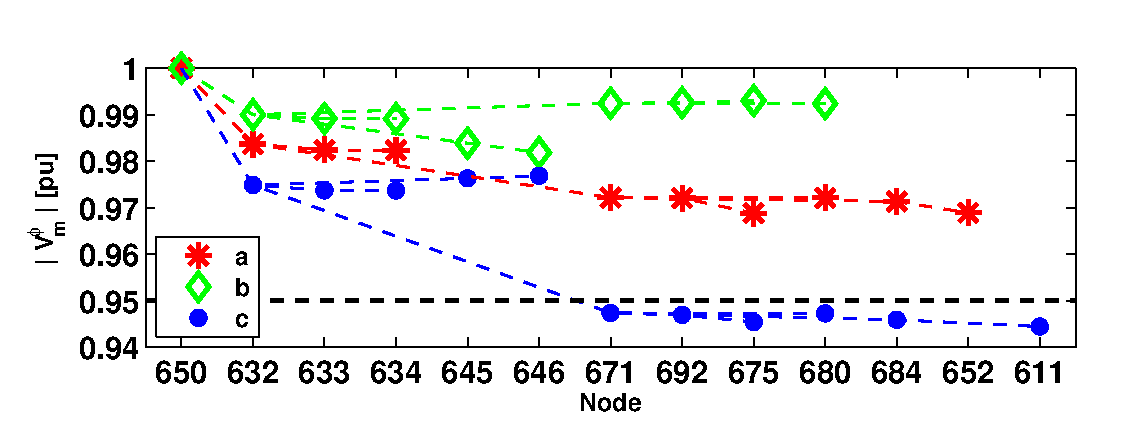
\includegraphics[width=0.49\textwidth]{s2bc.eps}
% 	\caption{Voltage profile of IEEE 13 node feeder without any DER control.}
% 	\label{fig:s2bc}
% \end{figure}


\label{sec:simulation_results}

\section{Conclusion}
\label{sec:conclusions}

Optimization of unbalanced power flow is a challenging topic due to its nonlinear and non-convex nature. While recent works on SDP relaxations  \cite{dall2012optimization} - \cite{dall2013distributed} have made OPF formulations for unbalanced systems possible, these approaches suffer from restrictions on the possible objectives and a high-dimensional geometrical complexity that impedes feasibility and uniqueness of the solutions.  In an effort to solve problems that cannot be addressed via SDP techniques, in this paper we sought to develop an approximate model for distribution power flow that could be subsequently incorporated into optimal power flow problems.  

To do so, we derived a generalized model of distribution system power flow that maps real and reactive power injections into squared voltage magnitude differences.  The resulting model, which we referred to as the \textit{Dist3Flow} equations, can be viewed as an extension of the \textit{DistFlow} \cite{baran1989optimal} equations to 3-phase unbalanced distribution systems.  As the \textit{Dist3Flow} model is nonlinear and not necessarily convex, we suggested two procedures to linearize the system into a form suitable for incorporation into OPF formulations.  The linearized power flow model, which we have referred to as the \textit{LinDist3Flow} system, is obtained by approximating the nonlinear components of the original equations.  

The first approximation procedure treated the ratio of voltages of different phases as a constant and neglected line losses.  The resulting \textit{LinDist3Flow} system was tested in an OPF with the objective of minimizing feeder-head real power.  Comparison of results obtained to a SDP formulation of the same problem revealed that the OPF driven by the \emph{LinDist3Flow} model achieved a solution whose objective function was within 0.2\% of the optimal value.
The second procedure for approximating the \textit{Dist3Flow} equations involved iterating over the nonlinear terms between successive runs of solving the power flow equations and then solving the OPF.  This approach was simulated in an OPF formulation with the objective of regulating and balancing system voltages, and was shown to increase accuracy compared to the previous approximation technique. 

 Although it is an approximation, the principle advantage of \emph{LinDist3Flow} model is that it enables an optimal power flow schemes where the constraints are linear and convex relaxations are not required.  As such, for strictly convex objectives with a non-empty feasible  set, the OPF will always find an optimal solution to the approximate problem.  As was mentioned previously, an OPF driven by the \textit{LinDist3Flow} model was able to solve a voltage balancing optimization, for which, by the knowledge of the authors, a SDP formulation does not exist.  Although the final solution is only approximate. The iterative method shows potential for further improving the accuracy gap between the linear and full nonlinear model, and future work will consider mathematical analysis to characterize this.

The feasibility of the \emph{LinDist3Flow} model can be exploited in OPF formulations with a variety of relevant objectives, such as voltage balancing, loss minimization, or economic dispatch. Our future work is aimed at exploring other useful applications of three phase unbalanced OPF such as voltage reference tracking or battery and electric vehicle charging. First, we will use our findings to extend the authors' work on optimal decentralized voltage regulation  \cite{sondermeijer2015regression}, developed for single-phase balanced networks, to 3-phase unbalanced systems. Furthermore, in a recent work, the authors developed a framework for distribution grid state estimation with limited sensing and forecasting information, using linearized power flow equations for single-phase systems \cite{dobbe2015real}. We aim to extend these results to unbalanced systems using the \emph{LinDist3Flow} equations.

  
\label{sec:conclusion}

%%%%%%%%%%%%%%%%%%%%%%%%%%%%%%%%%%%%%%%%%%%%%%%%%%
%% REFERENCES
%%%%%%%%%%%%%%%%%%%%%%%%%%%%%%%%%%%%%%%%%%%%%%%%%%

\bibliography{bibtex_DBA}
\bibliographystyle{IEEEtran}

\end{document}
